\documentclass[11pt]{article}

% --- Encoding and fonts ---
\usepackage[utf8]{inputenc}
\usepackage[T1]{fontenc}
\usepackage{mathpazo}
\usepackage{tikz}

% --- Language ---
\RequirePackage[english]{babel}

% --- Page layout ---
\RequirePackage[a4paper,margin=2.5cm]{geometry}
\RequirePackage{parskip}

% --- Footnotes ---
\newcommand{\affiliation}{\footnote}
\makeatletter
\def\@fnsymbol#1{\ensuremath{\ifcase#1\or *\or \dagger\or \ddagger\or \mathsection\or \|\or **\or \dagger\dagger \or \ddagger\ddagger \else\@ctrerr\fi}}
\makeatother

% --- Colour ---
\usepackage{xcolor}
\definecolor{cblue}{RGB}{0,70,140}
\definecolor{cgreen}{RGB}{100,140,0}
\definecolor{cred}{RGB}{190,10,50}

% --- Lists ---
\usepackage[shortlabels]{enumitem}
\setlist{itemsep=0ex,topsep=0ex,parsep=0.4ex}

% --- Mathematical packages ---
\usepackage{amsmath,amsfonts,amssymb,amsthm,mathtools,thmtools,thm-restate,bbm,centernot}

% --- Hyperlinks ---
\usepackage[hyphens]{url} % Line breaking of urls
\usepackage[hidelinks,colorlinks,pagebackref]{hyperref} % colouring of hyperlinks and backreferences in bibliography; must be loaded after url
\hypersetup{citecolor=cgreen,linkcolor=cblue,urlcolor=cblue}
\usepackage[capitalise,nameinlink,noabbrev,compress]{cleveref} % References in the document; must be loaded after hyperref and amsmath

% --- Bibliography ---
\renewcommand*{\backrefsep}{, }
\renewcommand*{\backreftwosep}{, }
\renewcommand*{\backreflastsep}{, }
\renewcommand*{\backref}[1]{}
\renewcommand*{\backrefalt}[4]{
	\ifcase #1 Not cited.%
	\or $\uparrow$#2%
	\else $\uparrow$#2%
	\fi%
}

\theoremstyle{plain}
\newtheorem{theorem}{Theorem}[section]
\newtheorem{lemma}[theorem]{Lemma}
\newtheorem{claim}[theorem]{Claim}
\newtheorem{proposition}[theorem]{Proposition}
\newtheorem{observation}[theorem]{Observation}
\newtheorem{corollary}[theorem]{Corollary}
\newtheorem{conjecture}[theorem]{Conjecture}
\newtheorem{problem}[theorem]{Problem}
\newtheorem{remark}[theorem]{Remark}
\theoremstyle{definition}
\newtheorem{definition}[theorem]{Definition}

% make proof environment use bold font, including alternative header
\makeatletter
\renewenvironment{proof}[1][\proofname]
{\par\pushQED{\qed}
	\normalfont\topsep6\p@\@plus6\p@\relax\trivlist
	\item[\hskip\labelsep\bfseries#1\@addpunct{.}]
	\ignorespaces}
{\popQED\endtrivlist\@endpefalse}
\makeatother

% Replace symbol for empty set
\let\emptyset\varnothing
\newcommand{\eps}{\varepsilon}


\newcommand{\cH}{\mathcal{H}}
\newcommand{\R}{\mathcal{R}}
\newcommand{\bN}{\mathbb{N}}
\newcommand{\cO}{\mathcal{O}}
\newcommand{\dcol}{d_{\textrm{col}}}

\newcommand{\Forb}{{\rm Forb}}
\newcommand{\arr}{\xrightarrow[]{v}}
\newcommand{\arrind}{\xrightarrow[]{v-ind}}
\newcommand{\Rk}{\R_{ind}}

\newcommand{\val}{w}
\DeclarePairedDelimiter{\abs}{\lvert}{\rvert}
\DeclarePairedDelimiter{\ceil}{\lceil}{\rceil}



% Pictures

\usepackage[T1]{fontenc}
\usepackage{lmodern}
\usetikzlibrary{decorations.pathreplacing}
\definecolor{pink}{RGB}{185,0,122}
\definecolor{palepink}{RGB}{235,195,231}
\definecolor{cyanframe}{RGB}{132,218,218}
\definecolor{grayvertex}{RGB}{105,105,105}
\definecolor{lavender}{RGB}{226,224,251}
\definecolor{chosen}{RGB}{230,25,35}
\tikzset{vertex/.style={circle,inner sep=1.65pt,fill=grayvertex},
  chosen/.style={vertex,fill=chosen,inner sep=2.1pt},
  attachment/.style={draw=gray!55,line width=.45pt}}
\newcommand{\Fshape}[2]{%
 \fill[#1,rounded corners=12pt] (-.73,-1.48) rectangle (.85,1.50);
 \fill[#2,opacity=.32] (.24,.67) ellipse [x radius=.49,y radius=.72];
 \fill[#2,opacity=.32] (.34,-.08) ellipse [x radius=.45,y radius=.61];
 \fill[#2,opacity=.32] (.23,-1.03) ellipse [x radius=.40,y radius=.32];
 \node[font=\Large] at (-.45,-.18) {$F$};
}
\newcommand{\Fpoints}[2]{%
 \foreach \i/\x/\y in {1/.05/1.05,2/.38/.82,3/.28/.30,4/.48/-.13,5/.27/-.43,6/.12/-.91,7/.35/-1.15}{%
  \coordinate (#1-\i) at (\x,\y);
  \node[vertex,fill=#2] at (#1-\i) {};
 }
}






\title{Non-isomorphic graphs have distinct vertex-Ramsey classes}
\author{Maria Axenovich and Patrick Schmitteckert \affiliation{Institute of Algebra and Geometry, Karlsruhe Institute of Technology, Germany (\textsf{\href{mailto:maria.aksenovich@kit.edu}{maria.aksenovich@kit.edu}, \textsf{\href{mailto:patrick@schmitteckert.org}{patrick@schmitteckert.org})}}}}
\date{\today}

\begin{document}
    \maketitle

    \begin{abstract}
        For a graph $H$,  its $k$-colour  vertex Ramsey class is the set of all graphs $G$ such that any colouring of the  vertices of $G$ in $k$ colours results in a monochromatic (induced) copy of $H$. 
        We prove that for any $k$,  Ramsey classes of any  non-isomorphic graphs are distinct. 
            \end{abstract}
    
    \section{Introduction}
  For a graph $H$ and $k\in \bN$, let  the {\it $k$-colour vertex Ramsey class} for $H$, denoted $\R^k(H)$,  be the set of all graphs  $G$ such that for any colouring of the vertices of $G$ in $k$ colours there is a subgraph isomorphic to $H$, that we call a {\it copy of $H$},  with all vertices of the same colour.   Similarly, we define  $\R_{ind}^k(H)$ if the copy of $H$ in the above definition is an induced subgraph of $G$.  
  The fact that  $\Rk^k(H)$ is nonempty for every graph $H$ was first shown by Folkman \cite{Folk}, see also \cite{BR, DHKZ, LRV, NR} for results on vertex Ramsey theory. 
  In this note we prove that any two non-isomorphic graphs have different $k$-colour Ramsey classes. Here, we assume that all graphs considered   have at least one vertex.
 
 \begin{theorem}\label{main}
 For any two   non-isomorphic graphs  $H_1$ and $H_2$ and  any  positive integer $k$,   $\R^k(H_1) \neq \R^k(H_2)$ and $\R_{ind}^k(H_1) \neq \R_{ind}^k(H_2)$.
 \end{theorem}
 
 
The study of Ramsey classes is a fundamental area in discrete mathematics addressing quantitative and structural properties of graphs in these classes.
Most existing  research  on Ramsey classes has concerned the setting of  edge colourings. A main motivation of this note is a question by  Fox,  Grinshpun, Liebenau, Person, and Szab\'o \cite{F}, whether any two connected non-isomorphic graphs have distinct edge Ramsey classes. While this question remains open in general,  we answer the  analogous question in the positive  for vertex colourings and all, not only connected, graphs. In Section \ref{sec:notations} we give some notations and needed Ramsey-type properties. Theorem \ref{main} is proved in Section \ref{proof-main}.



   
 \section{Notation and Ramsey properties}\label{sec:notations}
Let $H=(V, E)$ be a graph. We denote its order  $|V(H)|$ by $|H|$, its size $|E(H)|$ by $||H||$, its complement by $\overline{H}$, and 
its independence number by  $\alpha(H)$. If $||H||\geq 1$, let $\beta(H)$ be the largest order of a block of $H$, that is, a maximal 2-connected subgraph or a bridge; if $||H||=0$, let $\beta(H)=1$. For two graphs $G$ and $H$, let $G\vee H$ denote their join, that is a graph obtained as a union of vertex-disjoint copies of $G$ and $H$ together with all possible edges between these two copies.
 We denote the set of all graphs with no induced copy of $H$ by $\Forb(H)$.
 
 
 {\bf Construction 1.} Let $H$ be a graph and $q$ be an integer at least $3$.  Consider an  $|H|$-uniform hypergraph $\cH$ of girth at least $q$ and chromatic number at least $k+1$. The existence of such a graph was first shown by Erd\H{o}s and Hajnal \cite{EH}.
 Let $G=G(H, q, k)$ be a graph on vertex set $V(\cH)$ that is a union of $|E(\cH)|$ copies of $H$ induced by respective hyperedges of $\cH$. 
 We have that $G\in \Rk^k(H)$ since any vertex-colouring of $G$ in $k$ colours  and thus of $\cH$ results in a monochromatic hyperedge of $\cH$, i.e., a monochromatic induced copy of $H$. Note that this copy is indeed induced since the girth condition ensures that any two hyperedges of $\cH$ intersect in at most one vertex.

The definition of $\Rk^k$ implies that  $\R_{ind}^k(H_1) \neq \R_{ind}^k(H_2)$ if and only if $\R_{ind}^k(\overline{H}_1) \neq \R_{ind}^k(\overline{H}_2)$.
Using Construction 1 with sufficiently large girth and complementation we see  that for any graph $H$  and any positive integer $k$, there is $G \in \R_{ind}^k(H)$ such that $\alpha(H)=\alpha(G)$.
  
   
For a graph $A$, we denote a pairwise vertex-disjoint union of $q$ copies of $A$ by $qA$.  For $k\geq 1$, we say that a graph $H$ has  the  {\it Ramsey repetition property} if for any  integer $q \geq1$ and every graph $A$,   $ qA\in\Rk^k(H)$ if and only if $A\in\Rk^k(H).$
 \begin{lemma}\label{repetition}
For any $k\geq 1$, a  graph has the Ramsey repetition property if and only if it is connected.
\end{lemma}

\begin{proof}
Fix $k\geq 1$.

Assume that $H$ is connected. Let $q\geq1$. If $A\in\Rk^k(H)$, then clearly $q A\in\Rk^k(H)$.
If $A\not\in\Rk^k(H)$, repeat a colouring of $A$ without a monochromatic $H$ 
on its disjoint copies. This implies that $q A\not \in\Rk^k(H)$. Therefore $H$ has a Ramsey repetition property.

Let $H$  be disconnected and have components $H_1,\ldots,H_t$, where $t\geq2$. Let
$L=H_1\vee\cdots\vee H_t$. Choose
$A\in\Rk^k(L)$ with $ \alpha(A)=\alpha(L)$.     Since $\alpha(A)=\alpha(L)=\max_i\alpha(H_i)<\sum_i\alpha(H_i)=\alpha(H)$,
$A$ contains no induced $H$, thus  $A\not\in \Rk^k(H)$. 
Consider  an arbitrary $k$-vertex colouring of $qA$, for $q=k(t-1)+1$.
Each copy of $A$ contains a  monochromatic
$L$, and $t$ of these have the same colour. Taking $H_i$ from the $i$th
of these $t$ distinct copies gives a monochromatic induced $H$.
Therefore $qA \in \Rk^k(H)$.
Thus $H$ has no Ramsey repetition property.
\end{proof}

 

   
   \section{Proof of Theorem \ref{main}}\label{proof-main}
   Let $H_1$ and $H_2$ be two non-isomorphic graphs. If $k=1$, we have that $H_i\in \Rk^1(H_i)$, $i\in \{1,2\}$,  thus $\Rk^1(H_1)\neq \Rk^1(H_2)$ and  $\R^1(H_1)\neq \R^1(H_2)$.
   So, we assume that  $k\geq 2$.
   
   We shall first show that $\R^k(H_1) \neq \R^k(H_2)$. If $k=1$, we have that $H_i\in \R^k(H_i)$, thus $\R^k(H_1)\neq \R^k(H_2)$. Let $k\geq 2$.
   Assume first that $|H_1|\neq |H_2|$.  If $n=|H_1|<|H_2|$, let  $G=K_{k(n-1)+1}$.  By pigeonhole principle we see that $G\in \R^k(H_1)$. On the other hand, $G\not\in \R^k(H_2)$ because one can assign $k$ colours to the vertices of $G$ such that each colour class has size at most $n$.
   Now, assume that $|H_1|=|H_2|=n$. Since $H_1$ and $H_2$ are not isomorphic, without loss of generality assume that $H_1$ is not a subgraph of $H_2$.
   Let $G=H_2\vee K_{(k-1)(n-1)}$. To see that  $G\in \R^k(H_2)$, consider an arbitrary vertex-colouring of $G$. At least $n$ vertices are of the same colour, say red. Then the set of $n$ red vertices induces 
   a graph $G''=G'\vee K_{n-\ell}$, for some $\ell\geq 0$, where $G'$ is a subgraph of $H_2$ on $\ell$ vertices. Thus, $G''$ contains $H_2$ as a subgraph.
   On the other hand, by colouring the vertices of $G$ inducing  $H_2$ red and colouring  the remaining vertices in other, $k-1$ colours, such that each of these colours is present on $(n-1)$ vertices,  one has no monochromatic copy of $H_1$.\\
 
 Next, we shall prove that $\R_{ind}^k(H_1) \neq \R_{ind}^k(H_2)$.  Assume otherwise, i.e., that $\R_{ind}^k(H_1) = \R_{ind}^k(H_2)$.
 By Lemma \ref{repetition} we see  that both $H_1$ and $H_2$ are connected or both of them disconnected. By complementation, we can  assume that 
both of them are connected. If one of $H_1$ or $H_2$, say $H_1$, is a single vertex graph, $K_1$,  then $K_1\in \Rk^k(H_1)\setminus \Rk^k(H_2)$, so we are done.  We assume that $H_1$ and $H_2$ are  non-isomorphic connected graphs each containing at least one edge. 

Observe that if $H$ is connected and has an edge, there is an independent set
$I\subseteq V(H)$ such that $\beta(H-I)<\beta(H)$.
Indeed, we can greedily select such an $I$ by starting with some block as a root  in the block-cutvertex tree and processing its blocks away from the root.
Choose one vertex in the root block. For each subsequent block, if its
attachment vertex has already been chosen, choose nothing; otherwise
choose any other vertex in that block. A new vertex has no earlier
neighbours except possibly the attachment vertex, so the chosen set $I$
is independent and meets every block. 


 Assume without loss of generality that $\beta(H_1)\geq \beta(H_2)$ and if $\beta(H_1)=\beta(H_2)$, then 
$|H_1|\geq |H_2|$. In particular  $H_2\in \Forb(H_1)$. Choose an independent set $I$ of $H_2$ such that for $F=H_2-I$, 
 $\beta(F)<\beta(H_2)\leq\beta(H_1)$. 
 
 
 \begin{figure}
\begin{center}
\scalebox{0.7}{

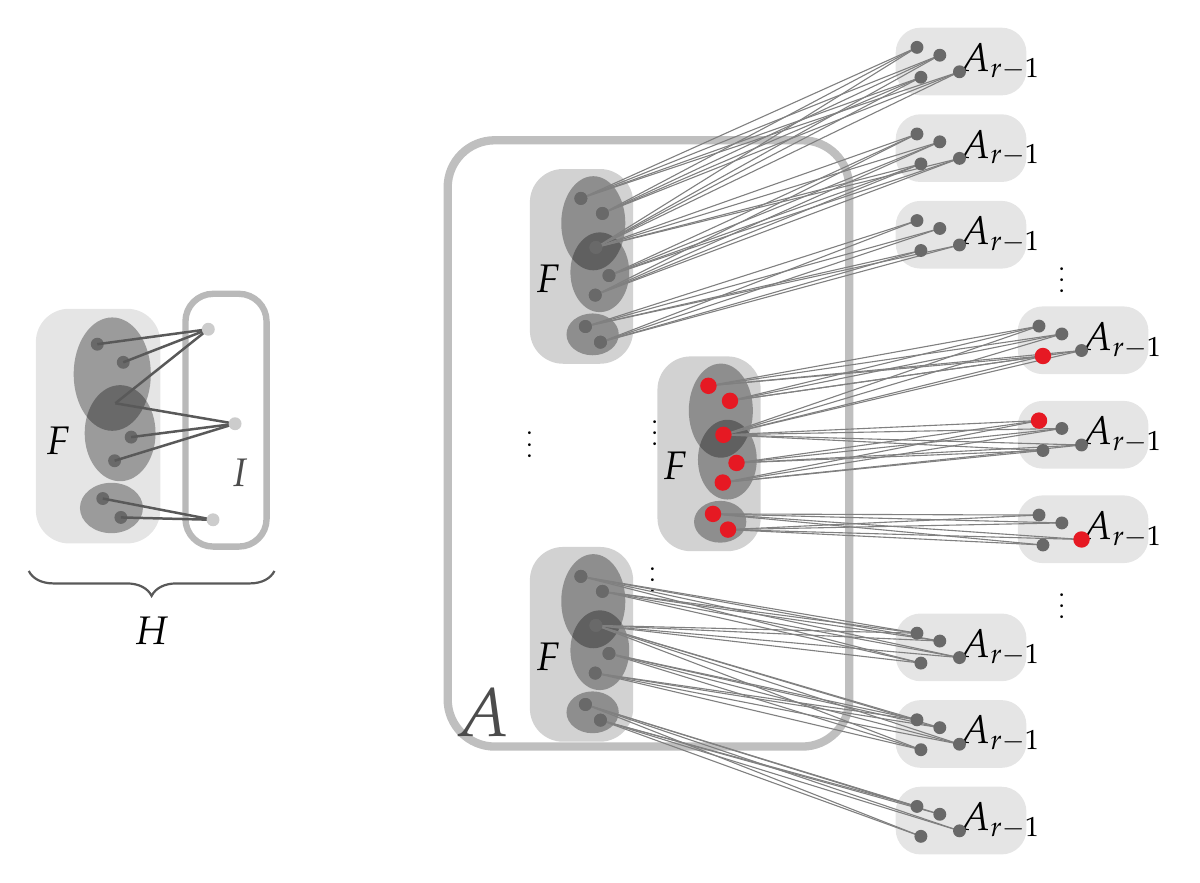
\begin{tikzpicture}[font=\small]
% The graph H, as in the sketch.
\begin{scope}[shift={(-4.6,0)},scale=1.0]
  \Fshape{gray!20}{black}
  \Fpoints{h}{grayvertex}
  \draw[gray!55,line width=2.3pt,rounded corners=10pt]
    (1.17,-1.52) rectangle (2.20,1.69);
  \node[font=\Large,text=black!70] at (1.86,-.58) {$I$};
  \coordinate (u1) at (1.46,1.24);
  \coordinate (u2) at (1.80,.04);
  \coordinate (u3) at (1.52,-1.18);
  \foreach \i in {1,2,3} {\draw[black!65,line width=.9pt] (h-\i)--(u1);}
  \foreach \i in {3,4,5} {\draw[black!65,line width=.9pt] (h-\i)--(u2);}
  \foreach \i in {6,7} {\draw[black!65,line width=.9pt] (h-\i)--(u3);}
  \foreach \i in {1,2,3} {\node[vertex,fill=black!20] at (u\i) {};}
  \draw[black!65,thick,decorate,decoration={brace,mirror,amplitude=9pt}]
    (-.82,-1.83)--(2.30,-1.83) node[midway,below=13pt,font=\Large,text=black] {$H$};
\end{scope}

% The three displayed copies of F in A.
\draw[black!25,line width=3pt,rounded corners=17pt]
  (-.1,-4.06) rectangle (5.0,3.64);
\node[font=\Huge,text=black!70] at (.35,-3.63) {$A$};

\begin{scope}[shift={(1.55,2.03)},scale=.83]
  \Fshape{gray!35}{black}
  \Fpoints{a}{grayvertex}
\end{scope}
\begin{scope}[shift={(3.17,-.35)},scale=.83]
  \Fshape{gray!35}{black}
  \Fpoints{b}{chosen}
\end{scope}
\begin{scope}[shift={(1.55,-2.77)},scale=.83]
  \Fshape{gray!35}{black}
  \Fpoints{c}{grayvertex}
\end{scope}

\node at (.94,-.12) {$\vdots$};
\node at (2.53,.03) {$\vdots$};
\node at (2.50,-1.84) {$\vdots$};

% Exactly three H-copies for each displayed F.
\foreach \prefix/\xx/\yone/\ytwo/\ythree in {
  a/6.35/4.64/3.54/2.44,
  b/7.90/1.10/-.10/-1.30,
  c/6.35/-2.80/-3.90/-5.00}{
  \foreach \idx/\yy in {1/\yone,2/\ytwo,3/\ythree}{
    \fill[gray!20,rounded corners=9pt] (\xx-.76,\yy-.43) rectangle (\xx+.90,\yy+.43);
    \node[font=\Large] at (\xx+.56,\yy) {$A_{r-1}$};
    \foreach \j/\dx/\dy in {1/-.49/.18,2/-.20/.08,3/-.44/-.20,4/.05/-.13}{
      \coordinate (\prefix-H\idx-\j) at (\xx+\dx,\yy+\dy);
    }
  }
  % Each entire H-copy receives the corresponding neighborhood in F.
  \foreach \s in {1,2,3}{\foreach \t in {1,2,3,4}{\draw[black!50] (\prefix-\s)--(\prefix-H1-\t);}}
  \foreach \s in {3,4,5}{\foreach \t in {1,2,3,4}{\draw[black!50] (\prefix-\s)--(\prefix-H2-\t);}}
  \foreach \s in {6,7}{\foreach \t in {1,2,3,4}{\draw[black!50] (\prefix-\s)--(\prefix-H3-\t);}}
  \foreach \idx in {1,2,3}{\foreach \j in {1,2,3,4}{\node[vertex] at (\prefix-H\idx-\j) {};}}
}

% Red representatives occur at different positions in the three selected copies.
\node[chosen] at (b-H1-3) {};
\node[chosen] at (b-H2-1) {};
\node[chosen] at (b-H3-4) {};

% Restore the seven F-vertices above the attachment lines.
\foreach \i in {1,...,7}{
  \node[vertex] at (a-\i) {};
  \node[chosen] at (b-\i) {};
  \node[vertex] at (c-\i) {};
}

\node at (7.70,1.97) {$\vdots$};
\node at (7.70,-2.17) {$\vdots$};
\end{tikzpicture}}
\end{center}
\caption{Construction of the graph $A_r$, $r\geq 2$ and a red copy of $H=H_2$.}
\label{figure}
\end{figure}

 
 First, we shall construct a graph $A\in \Forb(H_1)\cap \Rk^k(F)$.
 If $F$ has no edges, let $A$ be an edgeless graph on $k(|F|-1)+1$ vertices.
 If $F$ has edges, then $\beta(F)\geq 2$, thus $\beta(H_1)\geq 3$. Let $B$ be a block of $H_1$ on $\beta(H_1)$ vertices.
 Apply Construction 1 to build a graph $A=G(F, ||B||+2, k)$.
Since the girth of the underlying hypergraph is at least $||B||+2$ and $B$ is not contained in copies of $F$ placed in hyperedges of that hypergraph,  $A\in \Forb(B)$, thus $A\in \Forb(H_1)$.   By the property of Construction 1, $A\in \Rk^k(F)$. Thus $A\in \Rk^i(F)$ for all $i\in \{2,\dots,k\}$.

Next,  we recursively define graphs  $A_r$ for $r\in \{1,\dots, k\}$ such that $A_1:=H_2$ and for $r\geq 2$, $A_{r}\in \R_{ind}^{r}(H_2) \setminus \R_{ind}^{r}(H_1)$.
For $r\geq 2$,  we construct the graph $A_r$ based on $A_{r-1}$ as follows. Start with $A$. For every induced copy $\varphi(F)$ of
$F$ in $A$ and every $u\in I$, add a  copy $H_{\varphi,u, r-1}$ of $A_{r-1}$, such that these copies and $A$ are all pairwise vertex-disjoint. 
Make each vertex of $H_{\varphi,u,r-1 }$ adjacent to exactly those vertices of  $\varphi(F)$ that  correspond to the neighbours of $u$ in $H_2$, see Figure \ref{figure}.

We have that $A_r\not\in\Rk^r(H_1)$. Indeed, colour the vertices of $A$ red and the remaining vertices in other $r-1$ colours such that each copy of $A_{r-1}$ has no monochromatic induced copy of $H_1$. This colouring has no induced monochromatic copy of $H_1$.

On the other hand, $A_r\in \Rk^r(H_2)$.  To see this, consider an arbitrary  $r$-colouring of $V(A_r)$.  If some  added copy $H_{\varphi, u, r-1}$ of $A_{r-1}$ uses  at most  $r-1$ colours, it has a monochromatic induced copy of $H_2$. Otherwise, each such copy has all $r$ colours on its vertices.  Choose a monochromatic, say red,  induced  copy $\varphi(F)$ of $F$  in $A$,  and for each $u\in I$ choose a red
vertex of $H_{\varphi,u, r-1}$. Together these vertices and $\varphi(F)$ induce a red copy of $H_2$.

In particular, $A_{k}\in \R_{ind}^{k}(H_2) \setminus \R_{ind}^{k}(H_1)$, implying that  $\Rk^k(H_1)\neq \Rk^k(H_2)$ and  contradicting our assumption.
\qed



    \textbf{Acknowledgements.}  The proofs were obtained by alternating the authors' and ChatGPT 6.0's arguments.  The paper is written and checked by the authors.
 {\hypersetup{linkcolor=cred}
 \newcommand{\etalchar}[1]{$^{#1}$}
 
 
 
 \begin{thebibliography}{99}
 
\bibitem{BR}
J.~I.~Brown and V.~R\"odl,
\newblock A Ramsey type problem concerning vertex colourings,
\newblock {\em J.~Combin. Theory Ser. B} {\bf 52} (1991), 45--52.


\bibitem{DHKZ}
S.~Diskin, I.~Hoshen, M.~Krivelevich, and M.~Zhukovskii,
\newblock On vertex Ramsey graphs with forbidden subgraphs,
\newblock {\em Discrete Math.} {\bf 347} (2024), 113806.


\bibitem{EH}
P.~Erd\H{o}s and A.~Hajnal,
On chromatic number of graphs and set-systems,
Acta Mathematica Academiae Scientiarum Hungaricae
\textbf{17} (1966), 61--99.

\bibitem{Folk}
J.~Folkman,
\newblock Graphs with monochromatic complete subgraphs in every edge coloring,
\newblock {\em SIAM J. Appl. Math.} {\bf 18} (1970), 19--24.

 \bibitem{F} J. Fox, A. Grinshpun, A. Liebenau, Y. Person,  and T. Szab\'o, What is Ramsey-equivalent to a clique?, {\em J.~Combin. Theory Ser. B} 109 (2014), 120--133.

\bibitem{LRV}
T.~\L uczak, A.~Ruci\'nski, and B.~Voigt,
\newblock Ramsey properties of random graphs,
\newblock {\em J.~Combin. Theory Ser. B} {\bf 56} (1992), 55--68.

\bibitem{NR}
J.~Ne\v{s}et\v{r}il and V.~R\"odl,
\newblock Partitions of vertices,
\newblock {\em Comment. Math. Univ. Carolin.} {\bf 17} (1976), 85--95.

\end{thebibliography}
    
\end{document}



 
 
 
 
 
 
 
 
 
 
 
 
 
 
 
 
 
